\documentclass[aspectratio=169]{beamer}

\usepackage{basileabeam}
\usepackage[most]{tcolorbox}
\usepackage{subfig}
\usepackage{amsmath}
\usepackage{hyperref}

\setbeamercovered{invisible}
\addbibresource{presentation.bib}
% Notes:
%\pgfpagesuselayout{2 on 1}[a4paper,border shrink=5mm]
%\setbeamertemplate{note page}[plain]
%\setbeameroption{show notes on second screen=bottom}

\title              {Status Meeting - Application of Graph Learning to inverse problems}

\author     		{Cédric Mendelin}
\email				{cedric.mendelin@stud.unibas.ch}
\institute          {Department of Mathematics and Computer Science, University of Basel}

\date               {05.05.2022}

\ulogo        		{Template/header}
\ulistelement    	{Template/listelement}

\graphicspath{{Figures/}}

% Options:
%\totalNoSlidesDisabled % To turn off the total number of slides in the footer. Comment this if you want the total number of slides in the footer

%\headerSectionsDisabled % Comment this if you want a fancy header containing your sections.


\begin{document}

\AtBeginSection[]{%
  \frame<beamer>{ 
    \frametitle{Outline}   
    \tableofcontents[currentsection] 
  }
}

\begin{frame}[t,plain]
    \titlepage
\end{frame}

% \begin{frame}[t]{Outline}
%     \tableofcontents
% \end{frame}


%% Presentation content

% \section{Problem}	% You can also have slides prior to the first section or work entirely without sections.
\begin{frame}{Problem and Goal}
    \begin{itemize}
        \item Denoise observations
        \item Motivation from imaging (computed tomography, cryo-EM)
    \end{itemize}

    \pause
    \begin{block}{Input}
        $\mathcal{I}$: class of images (where $i \in \mathbb{R}^M$ with $M$ as image dimension.)
    \end{block}

    \begin{block}{Output}
        $$ denoiser:   (i + \eta) \mapsto i^* \approx i $$ 
        \center
        Where $i \in \mathcal{I}$ and $\eta \sim \mathcal{N}(0,\sigma^2) \in \mathbb{R}$.
    \end{block}

\end{frame}

\begin{frame}{Sinogram Denoiser}
    \begin{block}{}
        $$ forward : \text{radon transform} $$
        $$ backward : \text{filter back projection} $$
    \end{block}    
    
    \pause

    \begin{block}{Sinogram Denoiser}
        $$ denoiser_{sino}:  forward(i) + \eta \mapsto forward(i)^* \approx forward(i) $$ 
        $$ denoiser = backward ( denoiser_{sino}(forward(i) + \eta)) $$
        \center
        Where $i \in \mathcal{I}$ and $\eta \sim \mathcal{N}(0,\sigma^2) \in \mathbb{R}$.
    \end{block}
\end{frame}

\begin{frame}{GAT Denoiser}
    \begin{block}{GAT - Graph Attention Network}
        $$ GAT (A, \text{GAT args}) : \to \text{fixed angles} \to \text{k-nn circle graph} $$
    \end{block}    
    
    \pause
    \begin{alertblock}{Input Graph}
        \begin{itemize}
            \item Learning does work with circle graph
            \item Learning does not work with random (Erdős–Rényi) graph
        \end{itemize}
    \end{alertblock}

\end{frame}

\begin{frame}{GAT Denoiser - 2}
    \begin{block}{GAT - Graph Attention Network}
        $$ GAT (A, \text{GAT args}) : \to \text{fixed angles} \to \text{k-nn circle graph} $$
    \end{block}    

    \begin{block}{GAT Loss}
        $$ \mathcal{L}_1 = || forward(i) - denoiser_{sino}(forward(i) + \eta) ||_2 $$ 
        $$ \mathcal{L}_2 = || i - backward (denoiser_{sino}(forward(i) + \eta)) ||_2 $$ 
        \center
        Where $i \in \mathcal{I}$ and $\eta \sim \mathcal{N}(0,\sigma^2) \in \mathbb{R}$.
    \end{block}

\end{frame}


\begin{frame}{Current experiments - Toy images}
    \begin{itemize}
        \item Input images uniformly position shapes on image.
        \item Mostly fixed SNR, validation with same SNR
        \item Graph size = 1024 nodes, k-nn = 8
        \item Results with $\mathcal{L}_1$ available, few with $\mathcal{L}_2$.
    \end{itemize}

    \begin{figure}
        
\includegraphics[width=0.15\textwidth]{toyimage_01}
        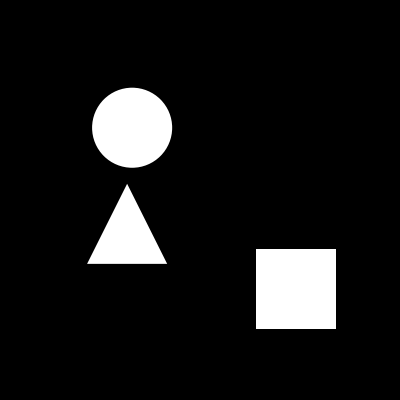
\includegraphics[width=0.15\textwidth]{toyimage_02}
        
\includegraphics[width=0.15\textwidth]{toyimage_03}
        
\includegraphics[width=0.15\textwidth]{toyimage_04}
        \caption{Example Toy images}
    \end{figure}
    
\end{frame}

\begin{frame}{Current Results - $\mathcal{L}_1$ vs $\mathcal{L}_2$}
    
    \begin{figure}
        
\includegraphics[width=0.15\textwidth]{noisy_fbp_5}
        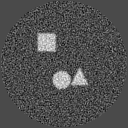
\includegraphics[width=0.15\textwidth]{noisy_fbp_0}
        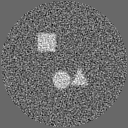
\includegraphics[width=0.15\textwidth]{noisy_fbp_n5}
        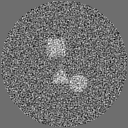
\includegraphics[width=0.15\textwidth]{noisy_fbp_n10}
        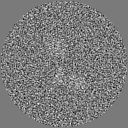
\includegraphics[width=0.15\textwidth]{noisy_fbp_n20}
        \caption{Noisy fbp with snr [5, 0, -5, -10 ,-20]}
    \end{figure}

    \begin{figure}
        
\includegraphics[width=0.15\textwidth]{denoised_fbp_5}
        
\includegraphics[width=0.15\textwidth]{denoised_fbp_0}
        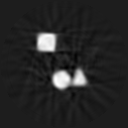
\includegraphics[width=0.15\textwidth]{denoised_fbp_n5}
        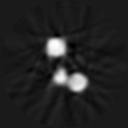
\includegraphics[width=0.15\textwidth]{denoised_fbp_n10}
        
\includegraphics[width=0.15\textwidth]{denoised_fbp_n20}
        \caption{Denoised fbp with snr [5, 0, -5, -10 ,-20]}
    \end{figure}
    
\end{frame}

\begin{frame}{Current Results - $\mathcal{L}_1$ vs $\mathcal{L}_2$ vs BM3D }

    \begin{figure}
        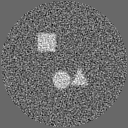
\includegraphics[width=0.15\textwidth]{noisy_fbp_n5}
        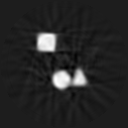
\includegraphics[width=0.15\textwidth]{denoised_fbp_n5}
        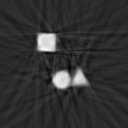
\includegraphics[width=0.15\textwidth]{denoised_ete_fbp_n5}
        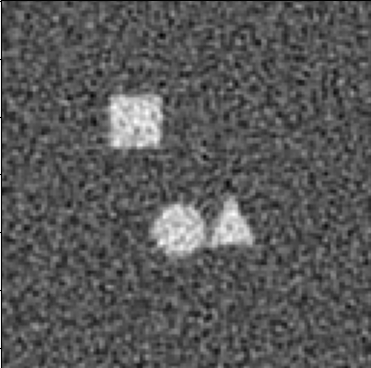
\includegraphics[width=0.15\textwidth]{bm3d_noisy_sino}
        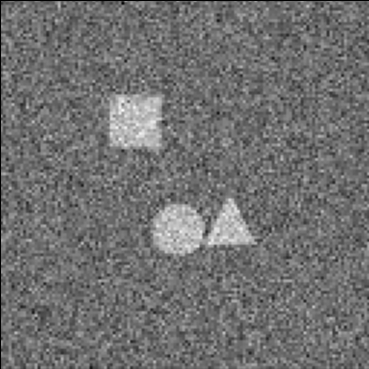
\includegraphics[width=0.15\textwidth]{bm3d_noisy_input}
        
        \caption{SNR -5 : noisy, denoised model $\mathcal{L}_1$, denoised model $\mathcal{L}_2$, BM3d noisy sinogram, BM3D noisy input}
    \end{figure}
    
\end{frame}

\begin{frame}{Some wandb reports}
    \begin{itemize}
        \item end-to-end: \url{https://wandb.ai/cedric-mendelin/end-to-end uniform generated toyimages scicore?workspace=user-cedric-mendelin}
        \item K-nn: \url{https://wandb.ai/cedric-mendelin/auto generated toyimages scicore knn/reports/Auto-toyimages-knn--VmlldzoxOTA4MjM2}
        \item 3d-Model: \url{https://wandb.ai/cedric-mendelin/bunnies scicore?workspace=user-cedric-mendelin}
        \item GAT parameters: \url{https://wandb.ai/cedric-mendelin/toy-images-input-size/reports/Toy-Images-Overview-Advanced-GAT--VmlldzoxNzczNDc0}
    \end{itemize}
    
    

\end{frame}

\begin{frame}{Final steps}
    \begin{itemize}
        \item Gather final results
        \item Write report
        \item Comparing with BM3D
    \end{itemize}
\end{frame}

\end{document}

